\chapter{Statistics in Photometry}

So far we've seen how the photometry should be done. But we haven't seriously discussed how to analize the uncertainties, i.e., the error-bars of each measurement such as magnitude. 

\section{Pixel-wise Uncertainty}
An object frame consist of at least bias, dark, flat, cosmic-ray, target's signal, and sky, as well as readout noise. For the $ j $-th pixel, they are denoted as:
\begin{itemize}
\item $ \tilde{N}_j $: the raw pixel value of the object frame in ADU.
\item $ B_j $: the bias in ADU.
\item $ D_j $: the dark in ADU.
\item $ F_j $: the flat in ADU (\textit{not necessarily} normalized; see \textbf{Note} at the end).
\item $ C_j $: the cosmic-ray in ADU.
\item $ I_j $: the object signal count in ADU.
\item $ S_j $: the sky signal in ADU.
\end{itemize}
In some cases, such as infrared detectors, the gain and readout noise may differ for each pixel, so I will denote gain and readout noise of the $ j $-th pixel as $ g_j \,[\mathrm{e/ADU}]$ and $ R_j \,[\mathrm{e}] $. Then we define the bias-subtracted pixel value
\begin{equation}
  N_j = \tilde{N}_j - B_j = D_j + (I_j + S_j + C_j) F_j
\end{equation}
Note that the dark is not affected by the flat value. Since this pixel value should follow a Poisson distribution, which is approximated as a Gaussian distribution,
\begin{equation}
  N_j 
    \simdot \mathcal{N} \left (
      N_j ,~ 
      \frac{N_j}{g_j} + \left (\frac{R_j}{g_j} \right )^2 
    \right ) ~.
\end{equation}

\subsection{Dark Estimation}
To estimate dark $ D_j $, you should have taken nearly tens of dark frames, and combined it. From the median value of the frames, you may have obtained the estimation of the dark $ \hat{D}_j $ (for brevity, I will just use $ D_j $ without the caret $ \hat{\cdot} $). During the combination, you can obtain the uncertainty of the dark at the $ j $-th pixel, $ \Delta D_j $, as
\begin{equation}
  \Delta D_j = \mathrm{sstd} (D_j^{i=1..N_\mathrm{Dark}}) 
    := \sqrt{ \frac{\sum_{i=1}^{N_\mathrm{Dark}} (D_j^{i} - \bar{D})^2}
      {N_\mathrm{Dark} - 1}} 
    \equiv \mathrm{std}(D_j^{i=1..N_\mathrm{Dark}}) 
      \times \sqrt{\frac{N_\mathrm{Dark}}{N_\mathrm{Dark} - 1}} ~,
\end{equation}
where $ D_j^{i} $ is the dark current (ADU) of the $ j $-th pixel at the $ i $-th dark frame, $ \mathrm{sstd} $ and $ \mathrm{std} $ are the \textit{sample} standard deviation (\texttt{np.std(x, ddof=1)}) and standard deviation (\texttt{np.std(x)}) functions, respectively, and $ N_\mathrm{Dark} $ is the number of dark framses used. Here it is assumed $ D_j $ roughly follows a Gaussian distribution so that $ \mathrm{sstd} $ becomes an unbiased estimator\footnote{An unbiased estimator of a random variable $ X $, $ \hat{X} $ is defined such that the expectation value of $ \hat{X} $ is the same as the true value $ X_\mathrm{true} $.} of the true standard deviation. Note that you should \emph{not} divide it by the number of dark frames (such as Thm \ref{thm: clt}), because \textbf{what you will need is not the uncertainty of the \emph{mean} value, but the uncertainty of one pixel value that will have been added to the object frame}. 
%, and $ N_\mathrm{Dark} $ is the number of dark frames. This is based on the CLT (Thm \ref{thm: clt}). Note the strong point of the CLT helps us here: CLT holds regardless of the distribution of $ D_j^{i} $! Even if we don't know anything about its distribution, we can use CLT without caring about it.

Therefore, to the first order,
\begin{equation}
\begin{aligned}
  \tilde{O}_j = N_j - D_j 
    &\simdot \mathcal{N} 
      \left ( \tilde{O}_j,~ 
        \frac{N_j}{g_j} + \left (\frac{R_j}{g_j} \right )^2 + (\Delta D_j)^2 \right ) \\
  \mathrm{or}
    &\simdot \mathcal{N} 
        \left ( \tilde{O}_j,~ 
          \frac{\tilde{O}_j}{g_j} 
          + \frac{D_j}{g_j} 
          + \left (\frac{R_j}{g_j} \right )^2 
          + (\Delta D_j)^2 \right ) ~.
\end{aligned}
\end{equation}
Note that we have been using $ N_j/g_j = (\tilde{O}_j + D_j)/g_j $ term in $ \Delta N_j $. This makes sence only if the Poissonity of dark is assumed.

\subsection{Flat Estimation}
Unlike the dark current, which is a probabilistic electron generation, the flat, i.e., the pixel sensitivity, is a characterestic value of the detector and optics, so it should not change at each exposure. Therefore, following the CLT (Thm \ref{thm: clt}): 
\begin{equation}
  \Delta F_j 
    = \frac{\mathrm{sstd} (F_j^{i=1..N_\mathrm{Flat}})} {\sqrt{N_\mathrm{Flat}}}
    := \sqrt{ \frac{1}{N_\mathrm{Flat}}
       \frac{\sum_{i=1}^{N_\mathrm{Flat}} (F_j^{i} - \bar{F})^2}{N_\mathrm{Flat} - 1}} 
       \equiv \frac{\mathrm{std}(F_j^{i=1..N})}{\sqrt{N_\mathrm{Flat} - 1}} ~,
\end{equation}
where $ F_j^{i} $ is the flat frame pixel value (ADU) of the $ j $-th pixel at the $ i $-th flat frame, $ \mathrm{sstd} $ is the sample standard deviation function and $ N_\mathrm{Flat} $ is the number of the used flat frames. 

Generally speaking, $ F_j $ must be about $ 10^4 $ ADU or more, so that the signal-to-noise ratio from Poisson statistics is larger than about 100. Moreover, you should have obtained, say, $ N_\mathrm{flat} = 9 $, this will increase by a factor of 3. Therefore, the uncertainty in the flat $ \Delta F_j $, is around 0.1 \% order. In some observatories, people take hundreds of flats at one time to get flat as good as roughly 0.01 \% order, assuming it won't change over certain period of time.

Although there are mathematically known ratio distribution, i.e., the pdf of $ Z := X/Y $ where $ X, Y \sim \mathcal{N}(\mu_{X, Y}, \sigma_{X, Y}^2) $ and the covariance is zero, what we are interested in is only a rough estimation of the uncertainties\footnote{If you are interested in, see FiellerEC (1932) Biometrika, 24, 428; HinkleyDV (1969) Biometrika, 56, 635;  D\'{i}az-Franc\'{e}s+RubioFJ (2013) Statistical Papers, 54, 309, as well as \href{https://en.wikipedia.org/wiki/Ratio_distribution}{Wikipedia}. For the ratio of $ N_j/F_j $, i.e., when the denominator has so high signal-to-noise ratio, the distribution is roughly a Gaussian with $ \mathcal{N}(\mu_X, \sigma_X^2) $ as we assume in this section.}. From the propagation of error, 
\begin{equation}
\begin{aligned}
  O_j = \frac{N_j - D_j}{F_j} = I_j + S_j + C_j
    &\simdot \mathcal{N} 
      \left ( O_j,~ 
        O_j^2 \left [ 
        \left (\frac{\Delta \tilde{O}_j}{\tilde{O}_j} \right )^2 
        + \left (\frac{\Delta F_j}{F_j} \right )^2 \right ] \right ) ~.
\end{aligned}
\end{equation}
Substituting previously obtained distribution of $ \tilde{O}_j $,
\begin{equation}
  O_j 
    \simdot \mathcal{N} 
      \left ( O_j,~ 
        \frac{O_j}{g_jF_j} 
        + \frac{D_j}{g_j F_j^2} 
        + \left (\frac{R_j}{g_j F_j} \right )^2 
        + \left  (\frac{\Delta D_j}{F_j} \right )^2
        + O_j^2 \left (\frac{\Delta F_j}{F_j} \right )^2
        \right ) ~.
\end{equation}

%Note that this variance is also obtained by the following logic: $ F_j $ has too high signal-to-noise ratio, $ \Delta F_j / F_j \ll 1 $, we can just assume $ F_j $ is a perfectly known constant without any uncertainty. Then $ O_j = \tilde{O}_j / F_j \simdot \mathcal{N}(O_j, (\Delta \tilde{O}_j)^2 / F_j^2) $, which is what we have above.


\subsection{Final Pixel-wise Uncertainty}
Many times the $ C_j $ is removed by the so-called \emph{cosmic-ray rejection} algorithms. 
\begin{thm}[Pixel-wise Error]
The final, cosmic-ray removed pixel value will follow
\begin{equation} \label{eq: pix error}
\begin{aligned}
  O_j^\mathrm{cr} = \frac{N_j - D_j}{F_j} - C_j = I_j + S_j 
    &\simdot \mathcal{N} 
      \left ( O_j^\mathrm{cr},~ 
        \frac{O_j}{g_jF_j} 
        + \frac{D_j}{g_j F_j^2} 
        + \left (\frac{R_j}{g_j F_j} \right )^2 
        + \left (\frac{\Delta D_j}{F_j} \right )^2 
        + O_j^2 \left (\frac{\Delta F_j}{F_j} \right )^2
        \right ) \\
    &\simdot \mathcal{N} 
      \left ( O_j^\mathrm{cr},~ 
        \frac{N_j}{g_jF_j^2} 
        + \left (\frac{R_j}{g_j F_j} \right )^2 
        + \left  (\frac{\Delta D_j}{F_j} \right )^2 
        + O_j^2 \left (\frac{\Delta F_j}{F_j} \right )^2
        \right ) 
\end{aligned}
\end{equation}
Here, $ O_j $ is the bias, dark, and flat corrected pixel value before the cosmic-ray removal, while $ N_j $ is only bias-subtracted pixel value. Usually the uncertainty from the estimation for $ C_j $ is ignored as it is too difficult to estimate. 
\end{thm}

In practical application, the following approximations may be used:
\begin{enumerate}
\item Calculating the $ \Delta D_j $ term all the time is annoying, and moreover, it is likely for most pixels $ \Delta D_j \ll \Delta O_j $, except for hot/bad pixels\footnote{Bad pixels must be masked properly prior to any sane calculation, as they are known to be ``wrong'' data. This is usually provided as a pixel mask file (e.g., \texttt{.bpm} file) by the observatory.}. Therefore, people just ignore it and set it to 0.  Theoretically, however, $ \Delta D_j > (R_j/g_j) $, because $\Delta D_j = \mathrm{sstd} (D_j^{i}) $ and $ D_j^{i} \simdot \mathcal{N} \left (D_j^{i},~ D_j^{i}/g_j + (R_j/g_j)^2 \right ) $. Therefore, a more reasonable approximation, or the lower limit of the uncertainty, would be $ R_j/g_j $. 
\item Frequently, $ \Delta F_j/F_j $ is much smaller than $ \Delta \tilde{O}_j/\tilde{O}_j $ (or we can increase $ N_\mathrm{Flat} $ to force that this holds), so the flat-error term is negligible. StetsonPB, for instance, asked the user to give a constant $ \Delta F_j/F_j \equiv \sigma_F $ for all pixels, such as 0, 0.01, or 0.0075, in \texttt{DAOPHOT}.
\item Many times we use the normalized flat (for more discussion, see below) such that its mean or median is 1, so $ F_j \sim 1 $ for all pixel. Then all $ F_j $ in \cref{eq: pix error} can be just ignored.
\item The $ D_j $ term is negligible for many times. It is not negligible only for hot pixels where $ D_j \gg 1 $, but likely the observer did not put the target of interest at where hot pixels present. Moreover, state-of-the-art CCDs, such as Subaru FOCAS for instance, has too small dark current $ D_j < 0.1 \,\mathrm{e/s} $. Therefore, most important parts in the object frames will have negligible $ D_j $ compared to $ O_j^\mathrm{cr} $. Therefore, this term is also ignored many times.
\end{enumerate}

Summarizing, \cref{eq: pix error} is approximated as
\begin{equation} 
\begin{aligned}
  O_j^\mathrm{cr} 
    &\simdot \mathcal{N} 
      \left ( O_j^\mathrm{cr},~ 
        \frac{O_j}{g_jF_j} 
        + \frac{D_j}{g_j F_j^2} 
        + \left (\frac{R_j}{g_j F_j} \right )^2 
        + \left  (\frac{\Delta D_j}{F_j} \right )^2 
        + O_j^2 \left (\frac{\Delta F_j}{F_j} \right )^2
        \right ) \\
    &\simdot \mathcal{N} 
      \left ( O_j^\mathrm{cr},~ 
        \frac{O_j}{g_jF_j} 
        + \frac{D_j}{g_j F_j^2} 
        + 2 \left (\frac{R_j}{g_j F_j} \right )^2
        + \sigma_F O_j^2 
        \right ) \\
    &\simdot \mathcal{N} 
      \left ( O_j^\mathrm{cr},~ 
        \frac{O_j}{g_j} 
        + \frac{D_j}{g_j} 
        + 2 \left (\frac{R_j}{g_j} \right )^2
        + \sigma_F O_j^2
        \right ) \\
    &\simdot \mathcal{N} 
      \left ( O_j^\mathrm{cr},~ 
        \frac{O_j}{g_j} 
        + 2 \left (\frac{R_j}{g_j} \right )^2
        + \sigma_F O_j^2
        \right ) \\
\end{aligned}
\end{equation}
Most frequently people even drop the factor 2 and $ \sigma_F $, and write $ O_j^\mathrm{cr} \simdot \mathcal{N} \left ( O_j^\mathrm{cr},~ O_j/g_j + (R_j/g_j)^2 \right ) $. The first dropping ($ 2(R_j/g_j)^2 \rightarrow (R_j/g_j)^2 $) may be justified because one $ (R_j/g_j)^2 $ came from the uncertainty in dark, and we usually ignore anything from dark\footnote{Some high-spec observatories even skip taking dark frames (e.g., Subaru).}. 

\subsubsection{Note}
\textbf{The flat frames are frequently assumed to be normalized}, i.e., the mean or median of $ F_j $ values of the frame is around 1. In the generalized error estimation given in this book, this normalization is not important. However, astronomers (including all tasks of IRAF) have conventionally used a very simplified version of error estimation, that is, the Poisson component of the pixel error is approximated as $ \sqrt{O_j/g_j} $: $ O_j \simdot \mathcal{N} (O_j, O_j/g_j) $. Note the factor $ F_j $ is missing! The true signal-to-noise ratio is $ O_j / \Delta O_j \approx \sqrt{O_j / (g_j F_j)} $, while in this approximation, it is $ \sqrt{O_j / g_j} $. If the flat was normalized, $ F_j \sim 1 $, so these two are similar. If it were not normalized, however, the signal-to-noise ratio in this classical approximation will be underestimated by a factor of $ \sqrt{F_j} \sim \sqrt{10^4 \,(\mathrm{ADU})} = 100 $!! You will be calculating wrong uncertainty in that case.


From STSDAS package, \texttt{stsdas/pkg/hst\_calib/wfpc/noise/fitnoise.x}: noise = R if pixel value not positive, otherwise, $ \sqrt{R^2 + N/g + (N \times \texttt{scalen}/100)^2} $ where \texttt{scalen} is maybe an uncertainty of pixel (flat uncertainty?) in percentage.

%#################################################################################
%#										#
%# NOISEFUNC --	Calculate the square-root of the variance expected at the 	#
%#		given DN level, based upon the noise model parameters.  	#
%#										#
%#	Initial code:	7/91 by RAShaw						#
%
%real procedure noisefn(dn) 
%
%include	"nmcom.h"
%
%#  Calling argument
%real	dn		# Value of pixel in Data Numbers
%
%# Local variables
%real	tmp
%real	noise		# Function value
%
%begin
%	tmp = scalen / 100.
%	if (dn <= 0.) 
%	    noise = readn 
%	else
%	    noise = sqrt (readn * readn + dn / gain + dn * dn * tmp * tmp) 
%	return (noise)
%end


\subsection{Signal-to-Noise Ratio (SNR)}
\textbf{SNR} $ := \mathrm{signal}/\mathrm{noise} $, is an estimation of the quality of the data. Simply speaking, the signal is the sky subtracted aperture summation. On the other hand, noise is the square root of the aperture summation on the \textit{variance map} (the map of $ (\Delta O_j)^2 $).

\begin{ex}[Maximum pixel-wise SNR]
Consider a classic CCD, which loses linearity at around 60,000 ADU (bias subtracted value). Say gain is $ g_j = 1.0 $, there is neither readout noise ($ R_j = 0.0 $) nor dark ($ D_j = 0.0 $), and there is no flat pattern ($ F_j = 1.0 $, $ \sigma_F = 0 $). Then only the Poisson noise term remains and thus the maximum SNR of the pixel is 
\begin{equation}
  \mathrm{SNR}_\mathrm{max}^\mathrm{pixel} 
    \approx \frac{60000}{\sqrt{60000}} = \sqrt{60000} = 245 ~.
\end{equation}
Even if the CCD has high bias, lose linearity earlier, high gain, etc, you should always get $ \mathrm{SNR}_\mathrm{max}^\mathrm{pixel} \sim 250 $.
\end{ex}

\begin{ex}[Maximum photometric SNR]
Consider the same CCD and now you have a simple circular Gaussian star (i.e., perfect Gaussian PSF) in the image, almost saturated but not saturated. The peak value before the saturation will be roughly 60,000 ADU after the sky subtraction. That is, this star has a radial profile $ I(r) \approx 60000 e^{-r^2/2\sigma^2} $. Depending on the seeing size and pixel scale, $ \sigma $ will change. 

For the case if the $ \mathrm{FWHM} \ll 1 \,\mathrm{pix} $, $ \mathrm{apsum} \approx 60,000 $, so the maximum SNR is $ \mathrm{SNR}_\mathrm{max}^\mathrm{star} \approx \mathrm{SNR}_\mathrm{max}^\mathrm{pixel} \sim 250 $.
 
If the FWHM is much larger than 1 pixel (say, 5 pixel), 60,000 is roughly the peak value of the Gaussian function. The integration of such Gaussian function is $ \sqrt{2 \pi} \sigma \times 60,000 \sim 60,000 \times \mathrm{FWHM} $, where FWHM is in pixel unit (note that $ \sqrt{2\pi}\sigma = 2.51 \sigma \approx \mathrm{FWHM} $). Therefore, 
\begin{equation}
 \mathrm{SNR}_\mathrm{max}^\mathrm{star} 
 \approx \frac{60000 \mathrm{FWHM}}{\sqrt{60000 \mathrm{FWHM}}}
 \sim 250 \sqrt{\mathrm{FWHM}}
\end{equation}

Otherwise, $ \int_{-0.5}^{0.5}\int_{-0.5}^{0.5} I(x, y) dx dy = 60,000 $, so it is a bit complicated to calculate (you may use the fact that the integration of Gaussian function is analytically expressed using erf). But you may simply use the above rule-of-thumb to check the maximum SNR.

In reality, uncertainty in sky, dark, readout noise will increase the noise and thus decrease the SNR. Gain larger than unity will have an effect of increasing SNR by factor of $ \sqrt{g} $. The PSF usually have longer tail than Gaussian, and this will increase the SNR.
\end{ex}

The magnitude system used in astronomy uses the logarithmic scale. From Pogson's formula, $ I_1/I_2 = 10^{-0.4 \Delta m} $ for two objects having fluxes $ I_1 $ and $ I_2 $, and magnitude difference $ \Delta m $. When $ \Delta m $ is small, $ \Delta m $ is the fractional difference of the fluxes. For example, $ \Delta m = 0.01 $ means $ I_1/I_2 \approx 0.99 $ or the flux difference is 0.01 (1 \%). See \cref{fig:deltamag} for the validity of this approximation. 

\begin{figure} [ht!]
  \centering
  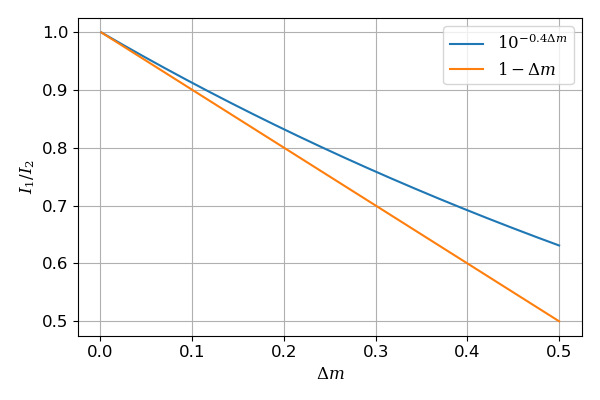
\includegraphics[width=0.5\linewidth]{figs/delta_mag}
  \caption{The delta magnitude plot.}
  \label{fig:deltamag}
\end{figure}

Differently put, if $ \Delta m =0.01 $ was the magnitude \textit{uncertainty} of the object, the uncertainty in flux is 1 \%, or $ \mathrm{SNR} = 100 $. Therefore, SNR can be directly converted to the magnitude uncertainty and vice versa. The $ \mathrm{SNR}_\mathrm{max}^\mathrm{pixel} = 250 $ translates to $ \Delta m \sim 1/250 = 0.004 $.


















